\chapter{Pipes and Filters}

\section{Summary}
Das "Pipes and Filters" Pattern bietet eine Struktur für Systeme die einen Stream von Daten verarbeiten, dabei wird jeder Verarbeitungsschritt als eine Filterkomponente dargestellt. Die Daten bewegen sich durch Pipes zwischen benachbarten Filtern.  
\section{Context}
Durch das "Pipies and Filters" Pattern werden folgende Forces adressiert: 
\begin{itemize}
	\item Zukünftige Systemerweiterungen sollten durch Austausch oder Neuordnung von Verarbeitungsschritten möglich sein
	\item Kleine Verarbeitungsschritte sind einfacher wiederverwendbar als grosse
	\item Nicht benachbarte Verarbeitungsschritte sollen keine Informationen teilen
	\item Es gibt verschiedene Quellen von Input Daten
	\item Es soll möglich sein Schlussresultate auf verschiedene Arten zu sichern
	\item Explizites Speichern von Zwischenresultate durch User ist fehleranfällig
	\item Man will die Möglichkeit nicht verwerfen, die Arbeitsschritte parallel zu verarbeiten
\end{itemize}


\section{Problem}
Gegeben ist ein System welches einen Stream von Daten verarbeiten muss. Das System wird von mehreren Entwicklern implementiert. Ausserdem lässt sich die generelle Aufgabe des Systems leicht in mehrere Teilaufgaben unterteilen, und die Wahrscheinlichkeit ist hoch, dass sich die Requirements ändern. Die Frage ist nun wie ein solches System designt werden soll damit mehrere Entwickler daran arbeiten können und flexibel auf Änderungen an den Requirements reagiert werden kann.
\section{Solution}
Mittels dem "Pipies and Filters" Pattern werden die Arbeitsschritte eines Systems in mehrere sequentiell verarbeitete Schritte unterteilt. Die Schritte sind durch den Data Flow durch das System verbunden, das heisst, die Output Daten eines Schrittes sind die Input Daten des nächsten. Jeder Arbeitsschritt wird als Filter Komponente implementiert. Ein Filter konsumiert und übermittelt inkrementell. Die Daten Source, die Filter und der Daten "Sink" werden durch sogenannte Pipes verbunden. 

\subsection{Structure}
Filter sind die Verarbeitungseinheiten einer Pipeline. Ein Filter hat drei Aufgaben:
\begin{enumerate}
	\item Anreichern von Daten durch Berechnungen und hinzufügen von Informationen
	\item Verfeinern von Daten durch Konzentration oder Extraktion von Daten
	\item Transformieren von Daten durch Übermittlung in einer anderen Repräsentation
\end{enumerate}
Ein Filter kann durch verschiedene Events ausgelöst werden:
\begin{itemize}
	\item Der darauffolgende Filter pullt die Output Daten
	\item Der vorangehende Filter pushed die Input Daten
	\item Üblicherweise pulling von Input Daten und pushen von Output Daten in einem Loop
\end{itemize}
Bei den ersten beiden Methoden handelt es sich um passive Filter, weil sie darauf warten getriggert zu werden. Bei der dritten Methode handelt es sich um einen aktiven Filter.

%\begin{figure}[H]
%  \centering
%  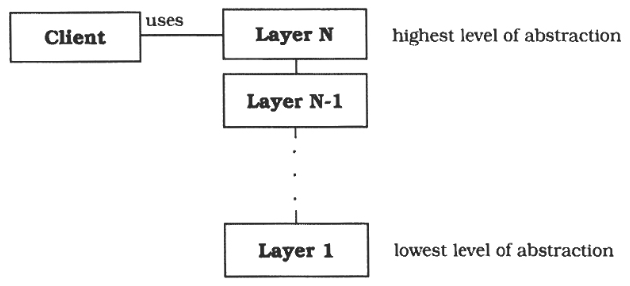
\includegraphics[width=0.8\textwidth]{figures/00-layers-1}
%  \caption{Illustration des Layer-Patterns}
%\end{figure}

\section{Consequences}
\begin{itemize}
    \pro{Keine Speicherung von Zwischenresultaten notwendig, jedoch weiterhin möglich}
    \pro{Flexibilität durch Filteraustausch}
    \pro{Flexibilität durch Neuordnung der Filterreihenfolge}
    \pro{Wiederverwendbarkeit von Filterkomponenten}
    \pro{Schnelles erstellen von Prototypen von Pipelines}
    \pro{Effizienz durch Parallelverarbeitung}
    \con{Teilen von Informationen über den State ist teuer}
    \con{Effizienzsteigerung durch Parallelverarbeitung ist meist eine Illusion}
    \con{Daten Transformations Overhead}
    \con{Error Handling}
    
\end{itemize}

\section{Known Uses}
\begin{itemize}
	\item UNIX
	\item CMS Pipelines
	\item LASSPTools
\end{itemize}

\section{Relationships}
\begin{itemize}
	\item \textit{Layers Pattern} Besser geeignet für Systeme welche zuverlässige Operationen benötigen, da es einfacher ist Error Handling zu implementieren
\end{itemize}

\section{Exam Questions}
\begin{itemize}
  \item Behauptung: dies ist eine Behauptung? (Lösung)
    \item Frage: Dies ist eine Frage? (Lösung)
\end{itemize}
